\documentclass{article}

\usepackage{fancyhdr}
\usepackage{extramarks}
\usepackage{amsmath}
\usepackage{amsthm}
\usepackage{amsfonts}
\usepackage{tikz}
\usepackage[plain]{algorithm}
\usepackage{algpseudocode}
\usepackage[shortlabels]{enumitem}
\usepackage{mathtools}
\usepackage{amssymb}
\usepackage{hyperref}
\usepackage{tikz}
\usepackage{pgfplots}

\usetikzlibrary{automata,positioning}

%
% Basic Document Settings
%

\topmargin=-0.45in
\evensidemargin=0in
\oddsidemargin=0in
\textwidth=6.5in
\textheight=9.0in
\headsep=0.25in

\linespread{1.1}

\pagestyle{fancy}
\lhead{\hmwkAuthorName}
\chead{\hmwkClassTime (\hmwkClassInstructor): \hmwkTitle}
\lfoot{\lastxmark}
\cfoot{\thepage}

\renewcommand\headrulewidth{0.4pt}
\renewcommand\footrulewidth{0.4pt}

\setlength\parindent{0pt}

%
% Create Problem Sections
%

\newcommand{\enterProblemHeader}[1]{
    \nobreak\extramarks{}{Problem \arabic{#1} continued on next page\ldots}\nobreak{}
    \nobreak\extramarks{Problem \arabic{#1} (continued)}{Problem \arabic{#1} continued on next page\ldots}\nobreak{}
}

\newcommand{\exitProblemHeader}[1]{
    \nobreak\extramarks{Problem \arabic{#1} (continued)}{Problem \arabic{#1} continued on next page\ldots}\nobreak{}
    \stepcounter{#1}
    \nobreak\extramarks{Problem \arabic{#1}}{}\nobreak{}
}

\setcounter{secnumdepth}{0}
\newcounter{partCounter}
\newcounter{homeworkProblemCounter}
\setcounter{homeworkProblemCounter}{1}
\nobreak\extramarks{Problem \arabic{homeworkProblemCounter}}{}\nobreak{}

\newcommand{\hmwkTitle}{Problem Set 1}
\newcommand{\hmwkDueDate}{January 26th, 2024}
\newcommand{\hmwkClass}{Introduction to Economics}
\newcommand{\hmwkClassTime}{ECON 101}
\newcommand{\hmwkClassInstructor}{Robert McDonough}
\newcommand{\hmwkAuthorName}{\textbf{Rushil Umaretiya}}

%
% Title Page
%

\title{
    \vspace{2in}
    \textmd{\textbf{\hmwkClass:\ \hmwkTitle}}\\
    \normalsize\vspace{0.1in}\small{\textbf{Due\ on\ \hmwkDueDate\ at 11:59pm}}\\
    \normalsize\text{Tuesday/Thursday 3:30-4:45, Genome Sciences 100}\\
    \vspace{0.1in}\large{\textit{\hmwkClassInstructor\ - \hmwkClassTime}}
    \vspace{3in}
}

\author{\hmwkAuthorName\\\small{rumareti@unc.edu}}
\date{}

\renewcommand{\part}[1]{\textbf{\large Part \Alph{partCounter}}\stepcounter{partCounter}\\}

%
% Various Helper Commands
%

% Useful for algorithms
\newcommand{\alg}[1]{\textsc{\bfseries \footnotesize #1}}

% For derivatives
\newcommand{\deriv}[1]{\frac{\mathrm{d}}{\mathrm{d}x} (#1)}

% For partial derivatives
\newcommand{\pderiv}[2]{\frac{\partial}{\partial #1} (#2)}

% Integral dx
\newcommand{\dx}{\mathrm{d}x}

% Alias for the Solution section header
\newcommand{\solution}{\textbf{\large Solution}}

\newcommand{\question}[1]{\pagebreak\section{Question #1}}

% Probability commands: Expectation, Variance, Covariance, Bias
\newcommand{\E}{\mathrm{E}}
\newcommand{\Var}{\mathrm{Var}}
\newcommand{\Cov}{\mathrm{Cov}}
\newcommand{\Bias}{\mathrm{Bias}}

\begin{document}

\maketitle

\question{1}

We apply the cost-benefit principle every day. As students, the choice to attend UNC involved big costs and (hopefully) benefits.

\begin{enumerate}[(a)]

    \item Attending UNC involves large out-of-pocket costs, which are listed
    on UNC's student aid website:
    \url{https://studentaid.unc.edu/current/costs/}.
    Using this site, find the total yearly cost of attending UNC as an
    in-state student.

    \begin{align*}
        \$27,036
    \end{align*}

    \item What is the North Carolina state minimum wage? Use the state minimum wage to calculate the foregone wages that you lose by attending UNC for the year.
        
    \begin{align*}
        \text{NC minimum wage } &= \$7.25\\
        \text{Foregone wages } &= \$7.25 \times 16 \frac{weeks}{semester} \times \text{ 2 semesters } \times \text{ 40 }\frac{hours}{week} = \$9,280
    \end{align*}

    \item Not all costs are measured in dollars! Describe some of the nonmonetary costs of spending a year at UNC.
    
    \begin{itemize}
        \item Time spent studying
        \item Stress and mental health impacts
        \item Social sacrifice (not being able to see friends and family)
        \item Physical health impacts (sleep, exercise, etc.)
        \item Delayed entry into the workforce
    \end{itemize}

    \item At UNC, most students graduate after 8 semesters (4 years). Setting aside the non-monetary costs, use the numbers you found
    above to calculate the opportunity cost of earning your degree. Ignore the possibility of student loans and aid, and pretend that
    you are paying out of pocket.

    \begin{align*}
        \text{Opportunity cost } &= \$27,036 \times \text{ 4 years } + \$9,280 \times \text{ 4 years }\\
        &= \$145,248
    \end{align*}

    \item Explain the cost-benefit principle in a sentence or two. Incorporating the numbers you found above, then explain your decision
    to attend UNC this year using the cost-benefit principle.

    The cost-benefit principle states that an individual should take an action if and only if the benefit of taking that action is greater than the cost of taking that action.

    For me, the average starting salary for a computer science major is ~\$80,000. After working for two years leaving college my benefit would outweigh the cost of attending UNC. I also enjoy the social aspect of college and the opportunity to learn new things. 

\end{enumerate}

\question{2} Your car needs gas before you can go to work this morning. You
decide to go to the gas station that is out of the way, but where gas
is \$0.10/gallon cheaper than the gas station on the way to work. This
gets you into work 10 minutes later than going to the other gas station.
If your wage is \$20/hour and you have to purchase 20 gallons of gas,
was this worth it? Why or why not?

\begin{align*}
    \text{Money saved on gas } &= \$0.10 \times \text{ 20 gallons } = \$2.00\\
    \text{Cost of time } &= \$20.00 \times \frac{1}{6} \text{ hours } = \$3.33\\
    \text{Total benefit } &= \$2.00 - \$3.33 = -\$1.33
\end{align*}

According to the cost-benefit principle, this was not worth it. The cost of time outweighs the money saved on gas.

\question{3} Tanner and Jasmine are each capable of producing two services: walking dogs or cooking meals. Tanner can cook a meal for 6 people in
an hour, or walk 1 dog in an hour. Jasmine can cook a meal for 2
person in an hour, or walk 3 dogs in an hour. They each have 4 hours
available to use to cook meals or walk dogs.

\begin{enumerate}[(a)]
    \item Draw a production possibilities frontier showing Tanner's capacity to cook meals or walk dogs, then add another PPF showing Jasmine's ability to cook meals or walk dogs.
    
    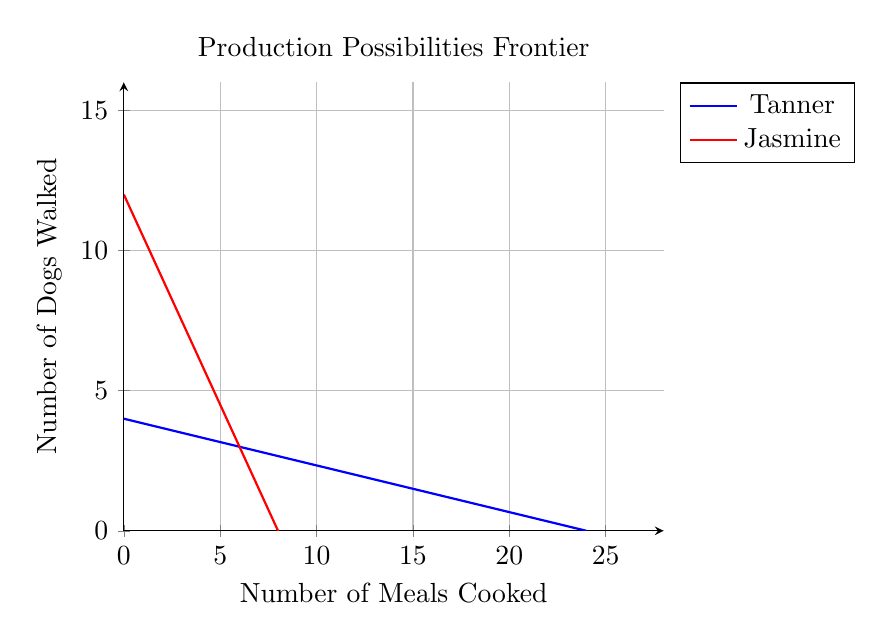
\begin{tikzpicture}
        \begin{axis}[
            title={Production Possibilities Frontier},
            xlabel={Number of Meals Cooked},
            ylabel={Number of Dogs Walked},
            xmin=0, xmax=28,
            ymin=0, ymax=16,
            axis lines=left,
            grid=both,
            legend pos=outer north east,
        ]
        
        % Tanner's PPF
        \addplot[domain=0:24, color=blue, thick] {4-1/6*x};
        \addlegendentry{Tanner}
        
        % Jasmine's PPF
        \addplot[domain=0:24, color=red, thick] {12-3/2*x};
        \addlegendentry{Jasmine}
        
        \end{axis}
        \end{tikzpicture}
        


    \item Label (including numbers) a point on Tanner's PPF that he could
produce at without trading. Do the same for a point on Jasmine's
PPF


    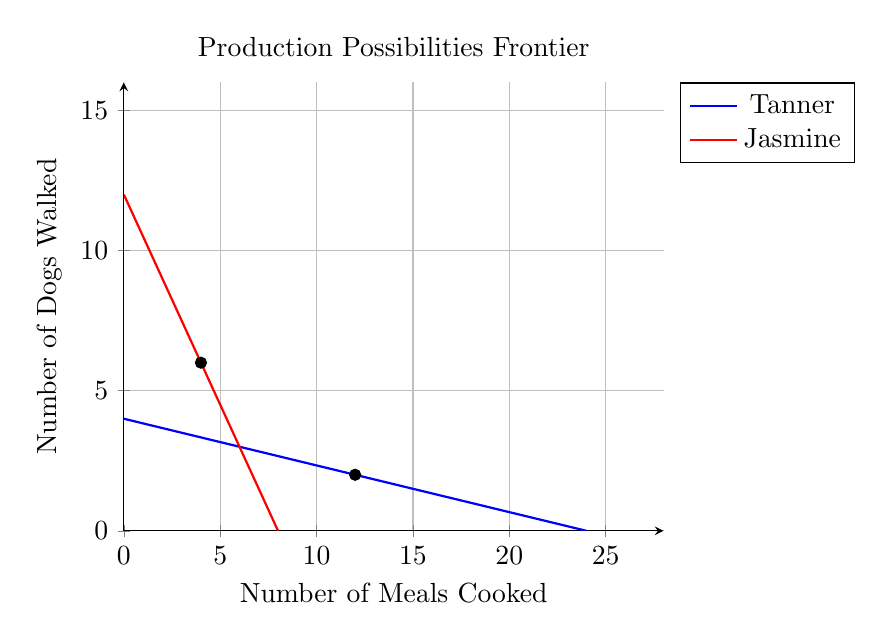
\begin{tikzpicture}
        \begin{axis}[
            title={Production Possibilities Frontier},
            xlabel={Number of Meals Cooked},
            ylabel={Number of Dogs Walked},
            xmin=0, xmax=28,
            ymin=0, ymax=16,
            axis lines=left,
            grid=both,
            legend pos=outer north east,
        ]
        
        % Tanner's PPF
        \addplot[domain=0:24, color=blue, thick] {-x/6 + 4};
        \addlegendentry{Tanner}
        
        % Jasmine's PPF
        \addplot[domain=0:8, color=red, thick] {-3*x/2 + 12};
        \addlegendentry{Jasmine}

        % Tanner's point

        \addplot[mark=*] coordinates {(12, 2)};

        % Jasmine's point  

        \addplot[mark=*] coordinates {(4, 6)};
        
        \end{axis}
        \end{tikzpicture}

        Tanner could produce 12 meals and walk 2 dogs without trading. Jasmine could produce 4 meals and walk 6 dogs without trading. This would be a total of 16 meals cooked and 8 dogs walked.
\pagebreak
    \item Who has the comparative advantage in cooking meals? Who
has the comparative advantage in walking dogs? Explain both
answers.


\begin{center}
    \begin{tabular}{ |c|c|c| } 
     \hline
     Opportunity Cost & Meals Cooked & Dogs Walked \\ 
     \hline
    Tanner & \(\frac{1}{6}\) dog & 6 meals \\
    \hline
    Jasmine & \(\frac{3}{2}\) dog & \(\frac{2}{3}\) meal \\
    \hline
    \end{tabular}
\end{center}


    Tanner has the comparative advantage in cooking meals because he can cook 6 meals in an hour while Jasmine can only cook 2 meals in an hour. Jasmine has the comparative advantage in walking dogs because she can walk 3 dogs in an hour while Tanner can only walk 1 dog in an hour.

    \item Tanner and Jasmine decide to specialize in producing one thing,
then trade. What will Tanner choose to produce and what will
Jasmine choose to produce. Explain your answer.

    Tanner will choose to produce meals because he has the comparative advantage in cooking meals. Jasmine will choose to produce walking dogs because she has the comparative advantage in walking dogs.

    \item What can we say about the price that Tanner and Jasmine would
both be willing pay to trade meals and dog walks?

    \textbf{Meals per dog walks:}\\
    Tanner would be willing to trade a meal for anything more than \(\frac{1}{6}\) of a dog walk, while Jasmine would be willing to trade a meal for anything less than \(\frac{3}{2}\) of a dog walk.\\

    \textbf{Dog walks per meal:}\\
    Tanner would be willing to trade a dog walk for anything less than 6 meals, while Jasmine would be willing to trade a dog walk for anything more than \(\frac{2}{3}\) of a meal.

    \item Suppose that before trading, Tanner and Jasmine each spent two
hours walking dogs and two hours cooking meals. What are the
gains to specialization and trade in this situation? Provide an
example for how the gains from trade could be distributed so
that Tanner and Jasmine each have more of each service than
before.

\begin{center}
    Before Trading\\
    \begin{tabular}{ |c|c|c| } 
     \hline
      & Meals Cooked & Dogs Walked \\ 
     \hline
    Tanner & 12 & 2 \\
    \hline
    Jasmine & 4 & 6 \\
    \hline
    \end{tabular}
\end{center}

Now, if both of them specialized, Tanner would cook 24 meals and Jasmine would walk 12 dogs. Let's say that Tanner and Jasmine agree to trade 2 meals for 1 dog walk, and they trade 12 meals for 6 dog walks. 

\begin{center}
    After Trading\\
    \begin{tabular}{ |c|c|c| } 
     \hline
      & Meals Cooked & Dogs Walked \\ 
     \hline
    Tanner & 12 & 6 \\
    \hline
    Jasmine & 12 & 6 \\
    \hline
    \end{tabular}
\end{center}

After trading, Tanner and Jasmine each have more than before trading, so there are gains to specialization and trade.
\pagebreak
    \item In your example for how the gains of trade could be distributed,
how much of each good are Tanner and Jasmine trading to one
another? Do these ”terms of trade” make sense, given what you
wrote in part (e)?

    Tanner and Jasmine are trading 2 meals for 1 dog walk. These terms of trade make sense because Tanner would be willing to trade a meal for anything more than \(\frac{1}{6}\) of a dog walk, while Jasmine would be willing to trade a meal for anything less than \(\frac{3}{2}\) of a dog walk. Tanner would be willing to trade a dog walk for anything less than 6 meals, while Jasmine would be willing to trade a dog walk for anything more than \(\frac{2}{3}\) of a meal. Therefore, Tanner and Jasmine would both be willing to trade 2 meals for 1 dog walk.
\end{enumerate}

\question{4}

Consider the market for a new physical copy of our textbook, \emph{Principles of Economics by Stevenson and Wolfers}. The instructors teaching large classes of ECON 101 at UNC all use this textbook. For each
of the following situations, decide if demand will shift, if supply will
shift, or if neither will shift. Then, draw a graph clearly illustrating
how supply or demand will shift.
\begin{enumerate}[(a)]
    \item The price of textbook ink increases.
    
    Since this situation affects production cost, the supply curve will shift to the left (decrease).

    \begin{tikzpicture}
        \begin{axis}[
            title={Supply Curve},
            ylabel={Price},
            xlabel={Quantity Supplied},
            yticklabel=\empty,
            xticklabel=\empty,
            xmin=0, xmax=10,
            ymin=0, ymax=10,
            axis lines=left,
            grid=none,
            legend pos=outer north east,
        ]
        
        \addplot[domain=0:10, color=blue, thick] {2*x};
        \addlegendentry{Old Supply}
        
        \addplot[domain=0:10, color=red, thick] {2*x + 2};
        \addlegendentry{New Supply}

        \addplot[mark=*] coordinates {(2.5,5)};
        \addplot[mark=*] coordinates {(1.5,5)};

        \end{axis}
    \end{tikzpicture}

    \item UNC mandates that all arts and science majors must take ECON
101.

    Since this situation affects the number of buyers, the demand curve will shift to the right (increase).

    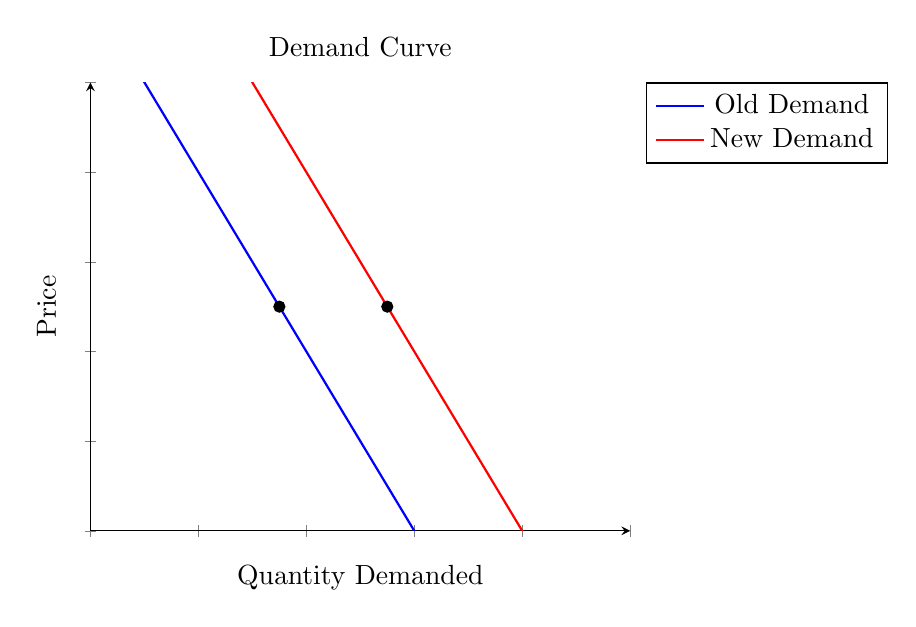
\begin{tikzpicture}
        \begin{axis}[
            title={Demand Curve},
            ylabel={Price},
            xlabel={Quantity Demanded},
            yticklabel=\empty,
            xticklabel=\empty,
            xmin=0, xmax=10,
            ymin=0, ymax=10,
            axis lines=left,
            grid=none,
            legend pos=outer north east,
        ]
        
        \addplot[domain=0:10, color=blue, thick] {-2*x + 12};
        \addlegendentry{Old Demand}
        
        \addplot[domain=0:10, color=red, thick] {-2*x + 16};
        \addlegendentry{New Demand}

        \addplot[mark=*] coordinates {(3.5,5)};
        \addplot[mark=*] coordinates {(5.5,5)};

        \end{axis}
    \end{tikzpicture}
    \pagebreak
    \item The price of the textbook rises.

    Since this situation affects the price of the good, there won't be a shift in either demand or supply curves, but a movement up the demand curve (decrease in quantity demanded) and a movement up the supply curve (decrease in quantity supplied).

    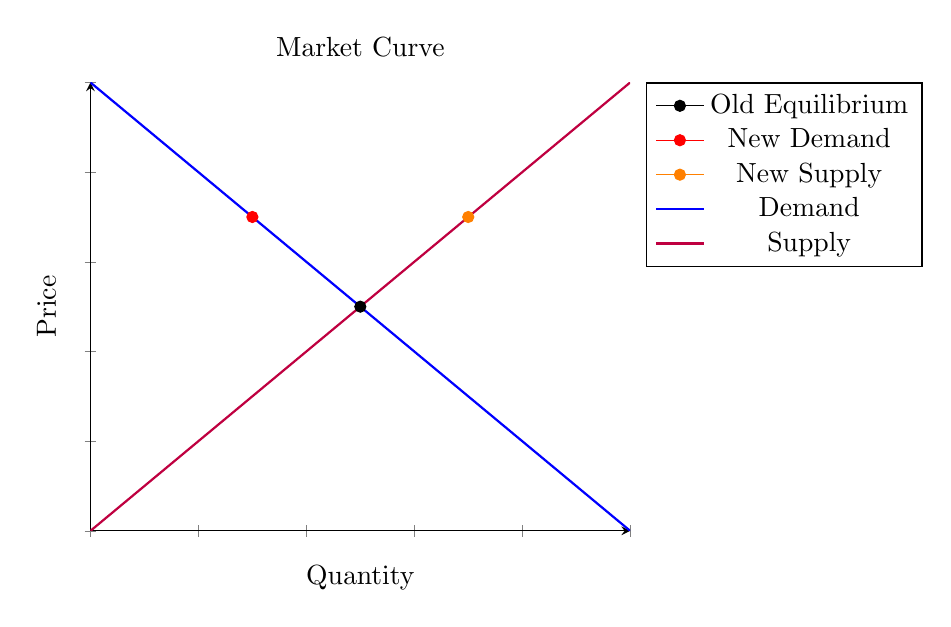
\begin{tikzpicture}
        \begin{axis}[
            title={Market Curve},
            xlabel={Quantity},
            ylabel={Price},
            yticklabel=\empty,
            xticklabel=\empty,
            xmin=0, xmax=10,
            ymin=0, ymax=10,
            axis lines=left,
            grid=none,
            legend pos=outer north east,
        ]
        
        \addplot[mark=*] coordinates {(5,5)};
        \addlegendentry{Old Equilibrium}

        \addplot[mark=*, color=red] coordinates {(3,7)};
        \addlegendentry{New Demand}

        \addplot[mark=*, color=orange] coordinates {(7,7)};
        \addlegendentry{New Supply}

        \addplot[domain=0:10, color=blue, thick] {-x+10};
        \addlegendentry{Demand}

        \addplot[domain=0:10, color=purple, thick] {x};
        \addlegendentry{Supply}

        \end{axis}
    \end{tikzpicture}

    \item The price of used copies of the old edition of the textbook decrease.
    
    Since this situation affects the price of a substitute good, the demand curve will shift to the left (decrease).


    \begin{tikzpicture}
        \begin{axis}[
            title={Demand Curve},
            ylabel={Price},
            xlabel={Quantity Demanded},
            yticklabel=\empty,
            xticklabel=\empty,
            xmin=0, xmax=10,
            ymin=0, ymax=10,
            axis lines=left,
            grid=none,
            legend pos=outer north east,
        ]
        
        \addplot[domain=0:10, color=blue, thick] {-2*x + 12};
        \addlegendentry{Old Demand}
        
        \addplot[domain=0:10, color=red, thick] {-2*x + 8};
        \addlegendentry{New Demand}

        \addplot[mark=*] coordinates {(3.5,5)};
        \addplot[mark=*] coordinates {(1.5,5)};

        \end{axis}
    \end{tikzpicture}

\end{enumerate}

\question{5}
Consider the daily market for a cup of coffee in Chapel Hill. Market demand for coffee is given by the equation \(P = 80 -\frac{1}{2}Q_d\), and market supply of coffee is given by \(P = \frac{Q_s}{38}\).

\begin{enumerate}[(a)]
    \item If the price of coffee is \$0, how many cups would buyers want to
consume? How many cups would sellers want to sell?

    \begin{align*}
        \text{If } P &= \$0\\
        0 &= 80 - \frac{1}{2}Q_d\\
        Q_d &= 160\\
        0 &= \frac{Q_s}{38}\\
        Q_s &= 0
    \end{align*}

It seems that buyers would want to consume 160 cups of coffee, but sellers would not want to sell any coffee.

    \item Calculate the price at which buyers would not want to buy any
coffee (i.e., \(Q_d = 0\)).

    \begin{align*}
        P &= 80 - \frac{1}{2}\cdot0\\
        P &= \$80
    \end{align*}

    Buyers would not want to buy any coffee at \$80.

    \item Calculate the equilibrium price of coffee and the quantity of coffee cups sold in Chapel Hill every day.
    
    \begin{align*}
        Q_d &= 160-2P\\
        Q_s &= 38P\\
        160-2P &= 38P\\
        160 &= 40P\\
        P &= \$4\\
        \\
        Q_d &= 160-2\cdot4\\
        Q_d &= 152
    \end{align*}

    The equilibrium price of coffee is \$4 and there are 152 cups of coffee sold in Chapel Hill every day.\pagebreak
    \item Draw a properly labeled diagram for the market for coffee in
    
Chapel Hill.

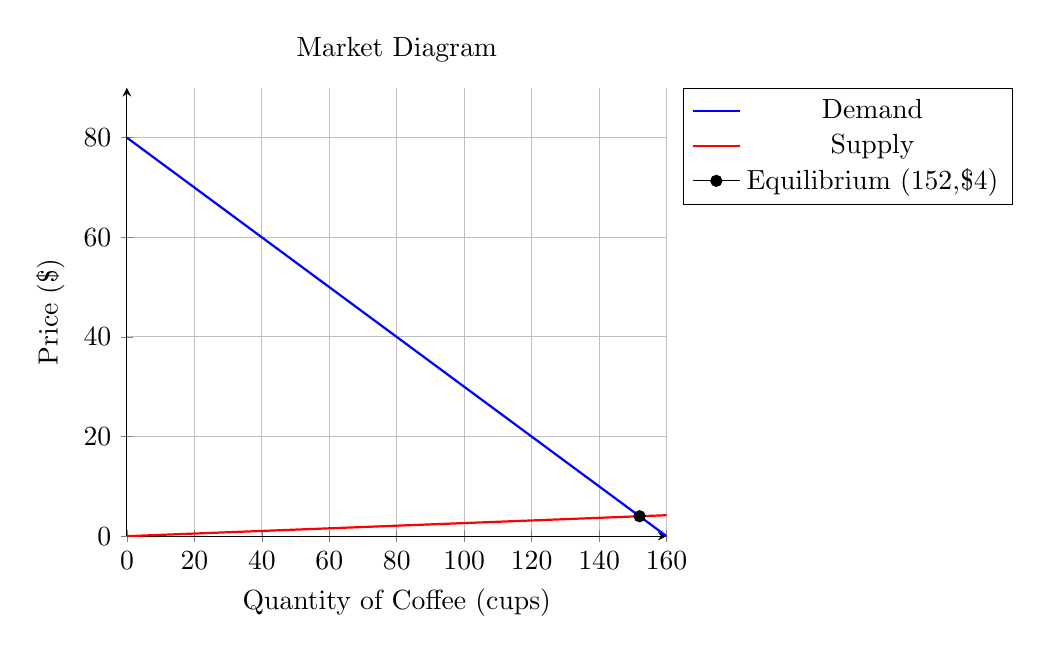
\begin{tikzpicture}
    \begin{axis}[
        title={Market Diagram},
        ylabel={Price (\$)},
        xlabel={Quantity of Coffee (cups)},
        xmin=0, xmax=160,
        ymin=0, ymax=90,
        axis lines=left,
        grid=both,
        legend pos=outer north east,
    ]
    
    \addplot[domain=0:160, color=blue, thick] {80-0.5*x};
    \addlegendentry{Demand}
    
    \addplot[domain=0:160, color=red, thick] {x/38};
    \addlegendentry{Supply}

    \addplot[mark=*] coordinates {(152,4)};
    \addlegendentry{Equilibrium (152,\$4)}

    \end{axis}
    \end{tikzpicture}

\end{enumerate}

\end{document}